% Noisy entanglement as a resource (notebook 54, Figure 1). One repeater node R between Alice and Bob.
% (1) Each segment produces noisy pairs (Werner pairs of fidelity F0), stored in quantum memories.
% (2) Distillation: two pairs of a segment -> one better pair (bilateral CNOT, measure the target pair, keep on
%     agreement, twirl), Section 7.
% (3) Swapping: a Bell measurement at R joins the two segments into one Alice-Bob pair; the Werner visibilities
%     multiply, v -> v1 v2, so the fidelity drops (Section 8).
% (4) Distil again at the next level, then certify: test a random sample of the delivered pairs with XX, YY, ZZ
%     correlations and keep the rest with the bound F >= F_hat - t (Section 9).
\documentclass[tikz,border=6pt]{standalone}
\usepackage{amsmath,amssymb}
\usetikzlibrary{arrows.meta,positioning,calc,decorations.pathmorphing}
\begin{document}
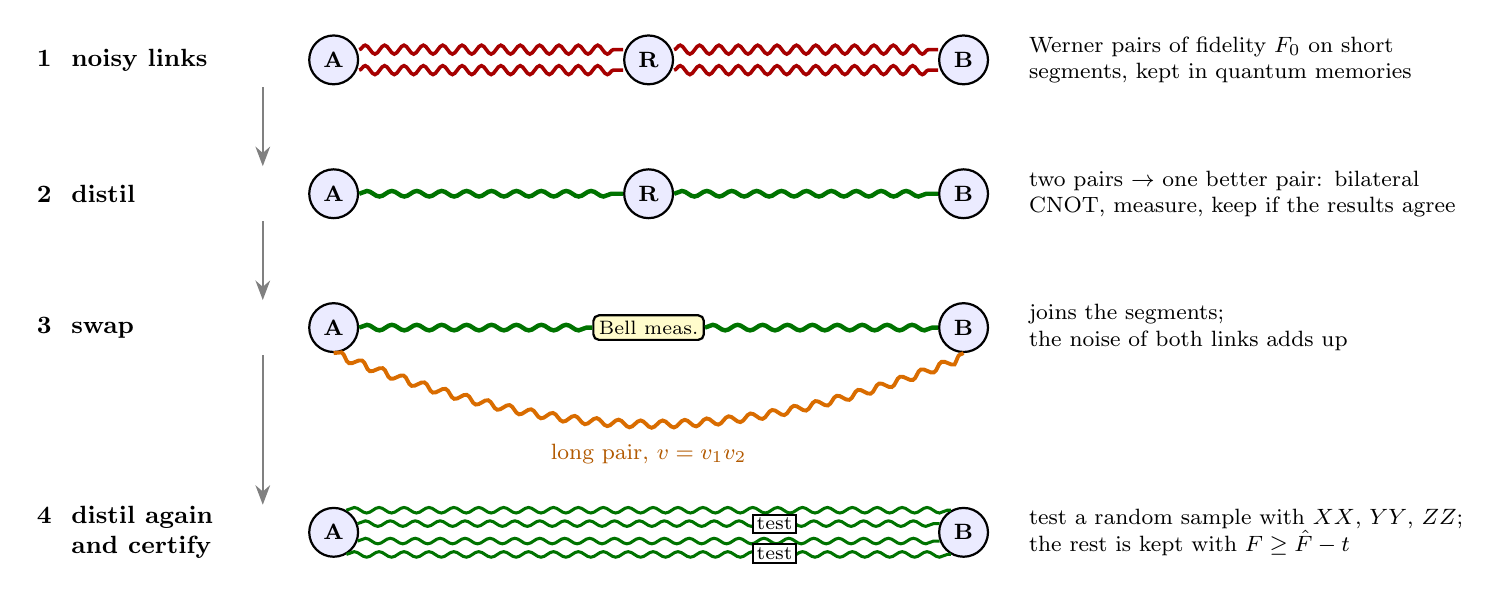
\begin{tikzpicture}[thick, >=Stealth, font=\small,
    nd/.style={circle, draw, fill=blue!8, minimum size=0.62cm, inner sep=0pt, font=\footnotesize\bfseries},
    noisy/.style={line width=1.3pt, red!65!black, decorate, decoration={snake, amplitude=1.6pt, segment length=7pt}},
    good/.style={line width=1.6pt, green!45!black, decorate, decoration={snake, amplitude=1.0pt, segment length=9pt}},
    mid/.style={line width=1.4pt, orange!85!black, decorate, decoration={snake, amplitude=1.3pt, segment length=8pt}},
    stp/.style={font=\small\bfseries, anchor=west, align=left},
    note/.style={font=\footnotesize, anchor=west, align=left, text width=5.6cm},
    bsm/.style={draw, rounded corners=2pt, fill=yellow!20, font=\scriptsize, inner sep=2pt}]
  % ---------------- row 1: elementary links ----------------
  \node[stp] at (-3.9,0) {1\ \ noisy links};
  \node[nd] (A1) at (0,0) {A}; \node[nd] (R1) at (4,0) {R}; \node[nd] (B1) at (8,0) {B};
  \draw[noisy] ($(A1.east)+(0,0.13)$) -- ($(R1.west)+(0,0.13)$);
  \draw[noisy] ($(A1.east)+(0,-0.13)$) -- ($(R1.west)+(0,-0.13)$);
  \draw[noisy] ($(R1.east)+(0,0.13)$) -- ($(B1.west)+(0,0.13)$);
  \draw[noisy] ($(R1.east)+(0,-0.13)$) -- ($(B1.west)+(0,-0.13)$);
  \node[note] at (8.7,0) {Werner pairs of fidelity $F_0$ on short\\ segments, kept in quantum memories};
  % ---------------- row 2: distillation per segment ----------------
  \node[stp] at (-3.9,-1.7) {2\ \ distil};
  \node[nd] (A2) at (0,-1.7) {A}; \node[nd] (R2) at (4,-1.7) {R}; \node[nd] (B2) at (8,-1.7) {B};
  \draw[good] (A2) -- (R2); \draw[good] (R2) -- (B2);
  \node[note] at (8.7,-1.7) {two pairs $\to$ one better pair: bilateral\\ CNOT, measure, keep if the results agree};
  % ---------------- row 3: swapping ----------------
  \node[stp] at (-3.9,-3.4) {3\ \ swap};
  \node[nd] (A3) at (0,-3.4) {A}; \node[nd] (B3) at (8,-3.4) {B};
  \node[bsm] (R3) at (4,-3.4) {Bell meas.};
  \draw[good] (A3) -- (R3); \draw[good] (R3) -- (B3);
  \draw[mid] (A3.south) to[out=-22, in=-158] (B3.south);
  \node[font=\footnotesize, orange!70!black] at (4,-5.0) {long pair, $v=v_1v_2$};
  \node[note] at (8.7,-3.4) {joins the segments;\\ the noise of both links adds up};
  % ---------------- row 4: distil again and certify ----------------
  \node[stp] at (-3.9,-6.0) {4\ \ distil again\\ \phantom{4}\ \ and certify};
  \node[nd] (A4) at (0,-6.0) {A}; \node[nd] (B4) at (8,-6.0) {B};
  \foreach \ang in {60,20,-20,-60} {
     \draw[good, line width=1.1pt] (A4.\ang) -- (B4.{180-\ang});
  }
  \foreach \ang in {20,-60} {
     \node[draw, fill=white, font=\scriptsize, inner sep=1.2pt] at (5.6,{-6.0+0.31*sin(\ang)}) {test};
  }
  \node[note] at (8.7,-6.0) {test a random sample with $XX$, $YY$, $ZZ$;\\ the rest is kept with $F\geq\hat F-t$};
  % ---------------- arrows between rows ----------------
  \foreach \a/\b in {0/-1.7,-1.7/-3.4,-3.4/-6.0} {
     \draw[->, black!50, line width=0.9pt] (-0.9,{\a-0.35}) -- (-0.9,{\b+0.35});
  }
\end{tikzpicture}
\end{document}
